% ------------------------------------------------------------------------
% -*-TeX-*- -*-Hard-*- Smart Wrapping
% ------------------------------------------------------------------------
\def\baselinestretch{1}

\chapter{Development}
\label{chapter:Development}

\def\baselinestretch{1.66}


%%% ----------------------------------------------------------------------

This chapter chronicles the development of the application, as well as testing of each individual element of the project as it is developed, in order to further refine it. This testing should not be confused with the testing section (chapter \ref{chapter:Testing}), which is larger scale testing of interactivity between system components, and of the system as a whole.

%%% ----------------------------------------------------------------------
\goodbreak

\section{Investigations}
\label{sec:Investigations}
This section chronicals experimentation undertaken to develop skills and basic \textcolor{red}{frameworks} using technologies identified as being useful to the project.

At the end of each of these sections, a series of aspects which will be included in the main project are outlined.

\subsection{Java and JSON}
\label{subSec:Java and JSON}
The goal of this investigation was to find a way that a Java back-end could be integrated with a 3D JavaScript based front-end which primarily uses three.js. \textcolor{red}{[SAY MORE ABOUT THIS]}

\subsubsection{17/12/2014: Version 1 \textcolor{red}{[READ THROUGH EACH VERSION, I THINK THERE IS A LOT OF REPETITION]}}
\label{subSubSection:Java and JSON: Lab 1}
This version establishes the use of csv files as storage of data about in-game elements. A test example, servers, is used, with servers.csv (in root/resources/data).

A java class was created for the retrieval of individual rows from servers.csv; ServerDataRetriever.java, which retrieves rows based on a supplied "key" string; All rows from the file are added to an array list, which is checked through iteratively using a for loop, which limited by the size of the array list: if a row string containing the key string is found in the array list, it is assigned as the output of the class's .getRow() method. 
ServerDataRetriever.java retrieves servers.csv's file path by getting its own runtime file path from the class loader, which it converts to a character array, removes all elements of it that do not correspond to the root of the application folder, and finally converts it to a string and concatenates the rest of the file path to it. 
Specifically, it does this adding all characters to the character array, then adding all but the last 26 of them to the file path string, with 26 being a known quantity of characters beyond the root folder in the class loader pathway for this file at run time.

For testing purposes, a server with the name (and key) "Type1" is retrieved, and is displayed on General\textunderscore MainPage.jsp as a java bean. As such, no JavaScript is used in this version because this version is intended only as a test of CSV files for data storage, and retrieval of data from them as rows.

\subsubsection{21/12/2014: Version 2}
\label{subSubSection:Java and JSON: Lab 2}
ServerRetriever was modified and renamed DataRetriever. Specifically, the getRow was modified to take one more string parameter, fileName, which is used to determine which file within the data folder to search for the specified row. This means that the one class can now be used to search any CSV file in the folder. 
DataRetriever was modified to retrieve a newly added header row from the CSV files using method ArrayList getHeaders(), which adds these as individual strings using a for loop and an if statement which iterates through the header row as a character array, concatenating characters to a string, which is added to the output array list whenever a comma is encountered in a character array. 
getHeaders is called from another new method, String convertToJSON(String), which itself is called by String getRow(). The method convertToJSON takes the row retrieved by getRow, adds it's CSV elements to an ArrayList in the same way that getHeaders does with the header row, and concatenates these elements with those returned by getHeaders into a JSON format string, where headers are assigned to values. 

DataRetriever's pathway assignment was abstracted to a string returned by a class called DataFolderFilePathPointer.java, which is a smaller class with a final string containing the absolute resources/data pathway for the system being used, allowing for easier set up of the project on different systems. 

As a test of the JSON value being retrieved, it is called as a java bean into \url{General_MainPage.jsp}, where it is called to be displayed on page in a pargraph with the id value "demo", having been parsed as a JSON object, with each element being called by it's respective header values, e.g. once added and JSONified, server "Type1" is called as obj.name.

\subsubsection{21/12/2014: Version 3}
\label{subSubSection:Java and JSON: Lab 3}
ServerRetriever was modified and renamed DataRetriever. Specifically, the getRow was modified to take one more string parameter, fileName, which is used to determine which file within the data folder to search for the specified row. This means that the one class can now be used to search any CSV file in the folder. 
DataRetriever was modified to retrieve a newly added header row from the CSV files using method ArrayList getHeaders(), which adds these as individual strings using a for loop and an if statement which iterates through the header row as a character array, concatenating characters to a string, which is added to the output array list whenever a comma is encountered in a character array. 
getHeaders is called from another new method, String convertToJSON(String), which itself is called by String getRow(). The method convertToJSON takes the row retrieved by getRow, adds it's CSV elements to an ArrayList in the same way that getHeaders does with the header row, and concatenates these elements with those returned by getHeaders into a JSON format string, where headers are assigned to values. 

DataRetriever's pathway assignment was abstracted to a string returned by a class called DataFolderFilePathPointer.java, which is a smaller class with a final string containing the absolute resources/data pathway for the system being used, allowing for easier set up of the project on different systems. 
Furthermore, DataRetriever's getRows and getHeaders methods were modified by having the strings where characters from their character arrays added to their respective string ArrayList objects, which overcame a bug where the last column header and row attribute were not being added to the JSON formatted string. 

For this version, \url{General_Mainpage.jsp} requests an entry from "servers.csv" with the name attribute "Type1". It retrieves it by using the getRows method of an object of class DataRetriever. 
This data is processed in the following way:

It is converted from a CSV row to a JSON format string by DataRetriever.
in seperate instances, the JSON format string is converted to a JSON object by the functions addToLocalStorage and processServer of JavaScript file JSTest.js.
In seperate instances, the JSON object is displayed on page by processServer, and retrieved from LocalStorage and displayed on page by function getRowFromStorage of JSTest.js ussing jQuery append functions.
In order to test the whole process of retrieving the row, converting it to JSON format, adding it to LocalStorage and retrieving it to the page from LocalStorage, three instances of the row are displayed on-page on \url{General_MainPage.jsp}: A Java scriptlet directly displaying the raw output of DataRetriever.getRow, the converted JSON object elements displayed by function processServer, and the JSON object retrieved from LocalStorage displayed by function getRowFromStorage.

\textbf{Page list:}
\begin{itemize}
\item \url{General_MainPage.jsp}\newline
In this version, this page contains on-page JavaScript which parses the returned string from DataRetriever.getRow as JSON, and displays its content on page.\newline

 This page references the following files:
\begin{itemize}
\item \textbf{Java classes and their methods:}

\begin{itemize}

\item \url{DataRetriever.java}

\begin{itemize}

\item \url{String}  \url{getRow(HttpServletRequest, HttpServletResponse, String, String)}\newline
Adds all rows from specified CSV file to an ArrayList, checks all entries in that ArrayList for a row with which contains the String parameter (the key), outputting such a row if it is found. This method finishes by calling the method convertToJSON.

\item \url{String} \url{convertToJSON(String)}\newline 
Adds all comma-seperated elements from the row, and uses a for loop and if statement to add all of the elements in that row to an array list by iteratively checking for commas in the input string as a character array, concatenating them to a string if a comma is not found, and adding that string to a string array if a comma is found. Next, this method calls the method getHeaders, and uses its String ArrayList content to form the row into a JSON format string.

\item \url{String} \url{getHeaders()}\newline 
This uses the same iterative for loop and if statement technique as convertToJSON to get all of the CSV format elements of the first row (the column headers) of the CSV file, which are used in convertToJSON to convert its string input to JSON format.

\end{itemize}

\item \url{DataFolderFilePathPointer}

\begin{itemize}
\item \url{String} \url{getPathway()}\newline
This returns the final string filePath, which is assigned by as the pathway to the web application's resources/data folder, which is called by classes which require this, such as DataRetriever.
\end{itemize}

\end{itemize}

\item \textbf{JavaScript files and their functions:}

\begin{itemize}

\item \url{JSTest}

\begin{itemize}

\item \url{processServer(row)}\newline
Takes a JSON format string (row) as its parameter (the output of DataRetriever.getRow()), which it converts to a JSON object, and retrieves elements with the JSON name tags "name", "x", "y", and "z", appending them to the "main" div of the page using the jQuery .append() method.

\item \url{processServerOnPage(row)}\newline
Works in the same way as processServer, appending the JSON elements as a string into div "demo" using document.getElementById("demo").innerHTML.

\item \url{addToLocalStorage(row)}\newline
Works in the same way as processServer, but adds the JSON elements to LocalStorage.

\item \url{getRowFromStorage(row)}\newline
Relies on addToLocalStorage, using the jQuery function .append() to add content from LocalStorage to the "main" div.
\end{itemize}
\end{itemize}
\end{itemize}
\end{itemize}

\subsection{Design decisions stemming from this investigation}
\label{subSec: Java and JSON: Design decisions stemming from this investigation}

The following decisions regarding the server-side Java conversion of data from CSV tables to JSON objects were made as a result of these investigations:

\begin{itemize}
\item JSON appears to be a data-interchange format which is particularly easy to handle client-side using reasonably simple JavaScript, and parsing data into JSON objects server side using Java objects is also relatively straightforward, therefore, JSON will be used in the project for the purpose of passing data from the server to the client.

\item Subsequent research has found that the current design of \url{General_MainPage.jsp} will not work when wrapped for mobile with PhoneGap because PhoneGap and Cordova cannot interpret Java Server Page files. However, PhoneGap can wrap all standard HTML5 file types (HTML, CSS and JavaScript), and it does allow for the passage of XML and JSON data between the server and the wrapped site. Therefore, the classes developed could still be used, but packaged into Java servlets called by HTML pages, rather than as JSP files \cite{PhoneGap:FAQs}. \textcolor{red}{[CITE PHONEGAP IN LIT REVIEW]}
\end{itemize}

\subsection{Three.js}
\label{subSec:Three.js}
This is a log of experiments using Three.js, with a mind to integrating the technology into the project, and including a 3D interface. The project is divided into a series of labs, which chronicle the changes made by session.

\subsubsection{Lab 1: 28/12/2015: First Three.js experiment}
\label{subSubSec:ThreeJSExperiments:Lab1}
his is a very simple HTML file displaying a rotating cube. It is a excercise in the basics of using Three.js for WebGL.

\subsubsection{Lab 2: 30/12/2014: .Obj file loader test: Local library access}
\label{subSubSec:ThreeJSExperiments:Lab2}
The first stage of this lab was to reverse engineer JavaScript data found associated with the Three.js OBJLoader demonstration \cite{ThreeJSObjLoader}, which features use of OBJLoader.js; part of the Three.js library which allows for the importation of .OBJ files for display through JavaScript.

This JavaScript file first copied and tested by changing the .OBJ file link from the one within the Three.js library specified in the demo for a model of a car uploaded by a user of tf3dm.com \cite{LarsenBMWObj}, and re-skinned with a plain white texture.

\subsubsection{Lab 3: 06/01/2015: .Obj file loader test: Remote library access \textcolor{red}{[REMOVE THIS, YOU'LL BE USING GIT]}}
\label{subSubSec:ThreeJSExperiments:Lab3}
A repeat of lab 2, attempting to reference the Three.js library from its location online, rather than locally

Unfortunatly, attempts to access the files as online resources through http://cdnjs.com/libraries/three.js/, my dropbox account and github all failed. As such, the large local three.js library and this project will be relocated as part of the DataCentreModelling project, in order to conserve space.

\subsubsection{Lab 4: 06/01/2015: Object animation tutorial}
\label{subSubSec:ThreeJSExperiments:Lab4}
Following of a tutorial at Tuts+ Code Tutorials \cite{Tuts+ThreeJS} to develop an animated cube object, without the need to import an external .obj file into the project.

\subsubsection{Lab 5: 08/01/2015: Camera animation tutorial modification}
\label{subSubSec:ThreeJSExperiments:Lab5}
Lab 4 is repeated, animating the camera to spin on it's Y axis, rather than the cube object.

\subsubsection{Lab 6: 12/01/2015: TrackballControl.js: A development of the page \newline``WebGL With Three.js: Basics"} 
\label{subSubSec:ThreeJSExperiments:Lab6}
A modification of the same Tuts+ Code Tutorial used in Lab 4 \cite{Tuts+ThreeJS}, exchanging pyramids for cubes.

This experiment is undertaken to explore the potential of TrackballControls.js within the Three.js library

This was tested both on a Windows 7 system, and an Android tablet. The windows testing revealed that clicking and dragging on any part of the page would pan the camera around the scene, and using the mouse-wheel would zoom the camera into the scene (forward for zooming in, backward for zooming out). The testing on the Android tablet revealed that touching and dragging on the page rotated the camera around the scene, pinching outwards with two fingers zoomed the camera out from the scene, pinching inwards with two fingers zoomed the camera into the scene, and dragging two fingers across the screen moved the camera along an axis relative to the 3D object.

\subsubsection{Lab 7: 12/01/2015: A single lit object viewed by a trackball controlled camera}
\label{subSubSec:ThreeJSExperiments:Lab7}
A development of the work in Lab 4 (and by extention http://code.tutsplus.com/tutorials/webgl-with-threejs-basics--net-35688), producing more of a blank canvas, with the ultimate goal of producing a template JavaScript file (or collection of files) to use in the DataCentreModelling project.

\subsubsection{Lab 8: 14/01/2015: A single lit, animated object viewed by a trackball controlled camera}
\label{subSubSec:ThreeJSExperiments:Lab8}
This features an .obj 3D object file imported into the scene using an OBJLoader class object, coloured with a plain white JPEG file, and illuminated from one side by a red spotlight. The scene is also observed by a camera controlled by a TrackBallConrols class object, allowing free movement, rotation and zooming of the camera relative to the scene.

\subsubsection{Lab 9: 15/01/2015: Lighting experiment}
\label{subSubSec:ThreeJSExperiment:Lab9}
An attempt was made to produce variable colour and three.js spotlights, controlled by HTML buttons linked to embedded JavaScript was made. This failed, and was postponed due to not being essential to the project.

\subsubsection{Lab 10: 21/01/2015: Implementation of three.js voxel painter at ``three.js webgl - interactive - voxel painter"}
\label{subSubSec:ThreeJSExperiments:Lab10}
This is an implementation of source code found at a Three.js demonstration, which displays a three.js based voxel painting canvas \cite{ThreeJSVoxelPainter}.

This implements the use of "voxels", or volumetric pixels, which are added as coloured cubes to a three dimensional grid plane. This makes an interesting potential basis for the data centre modelling application: This grid-plane system could be used, with the voxels replaced by 3D objects representing items being added to the data centre floor.

\subsubsection{Lab 11: 24/01/2015: Combination of three.js voxel painter with TrackballCamera.js}
\label{subSubSec:ThreeJSExperiments:Lab11}
This experiment brings together two different projects, Lab 7 (and by extension the three.js voxel painter demonstration \cite{ThreeJSVoxelPainter}), producing a 3D voxel painter, using a three.js roll-over mesh, a roll-over helper when the cursor passes over the mesh, and allowing a black 3D cube to be placed wherever the roll-over helper is when the mouse is clicked, and for the camera to be moved around the scene by the by clicking and dragging the cursor, making for intuitive control of the voxel painter, including camera relocation.

\subsubsection{Lab 12: 04/03/2015: Inclusion of 3D objects generated from JSON files into Lab-11}
\label{subSubSec:ThreeJSExperiments:Lab12}
This is a development of lab-11, replacing the Three.js BoxGeometry cubes placed on the grid with a 3D object imported from an external file, as was the case with lab-8 and before.

Unlike lab-8, the file used to generate the 3D cones placed by clicking on the grid is a JSON file rather than an .obj file; this is because it was found to be difficult to sucessfully cast the three.js .obj file loader class object, OBJLoader, into the framework that already existed in lab-11, where as the class which interprets JSON files as 3D objects, JSONLoader, is possible to integrate in the existing manner that BoxGeometry was.

\subsubsection{Lab 13: 05/03/2015: Decomposition of ThreeJSExperiments\textunderscore Lab12.js into an object-oriented structure}
\label{subSubSec:ThreeJSExperiments:Lab13}
This is a deelopment of lab-12, decomposing it into a single JavaScript file which call various JavaScript classes, each of which is contained within it's own JavaScript file. These classes each encapsulate a single aspect of the model, for example, RolloverCursor handles the drawing of the rollover cursor cube, and Skybox handles the drawing of the skybox.

Essentially, the classes are functions, and their operations are nested functions, while importation of functions into the namespace is handled as JavaScript inclusions within the HTML document calling them. The static context from which objects of these classes are constructed, and their operations are called is the un-encapsulated part at the beginning of the calling class (henceforth the main class, which in this context is ThreeJSExperiments Lab13.js. This idea follows from the tutorial at Scorchsoft.com \cite{ScorchSoftJavaScriptObjectOrientation}.

This lab includes a number of commits to a GIT repository, outlined below:

\begin{enumerate}
\item \textbf{07/03/2015: Commit ID a1ba56d:} Created the folder web/js/lab13 as a container for experimental changes to ThreeJSExperiments\textunderscore Lab12.js, which are then added to web/js/ThreeJSExperiments\textunderscore Lab13.js. ThreeJSExperiments \textunderscore Lab13a was created, which features all of the functionality required to draw the grid-plain decomposed into function draw of pseudo-class Grid. This approach to object-oriented programming in JavaScript was found at Scorchsoft.com \cite{ScorchSoftJavaScriptObjectOrientation}.

\item \textbf{07/03/2015: Commit ID aa241ba:} Further extended pseudo-class Grid within ThreeJSExperiments\textunderscore Lab13a.js with a constructor which is called by default, and commented-out code for private and public attributes.

\item \textbf{07/03/2015: Commit ID 7c758e2:} web/js/ThreeJSExperiments\textunderscore Lab13a.js is completed; all model-level architectural elements have been decomposed into pseudo-classes, with "draw" functions for their respective elements.

\item \textbf{07/03/2015: Commit ID 14f4e84:} The class CameraControls, which was formerly part of web/js/lab13/ThreeJSExperiments\textunderscore Lab13a.js, was migrated into it's own file at web/js/lab13/model/CameraControls.js, and is successfully called from web/js/lab13/ThreeJSExperiments\textunderscore Lab13b.js, which means that camera controls are handled by that class in that file when called as \newline var cam = new CameraControls(). The class CameraControls contains a constructor, which, in the context of JavaScript deployed in this manner, is a child-function which is called within the parent function (the class itself). This means that the object is fully initialised on construction.

\item \textbf{08/03/2015: Commit ID 6dc2c35:} All code from web/js/lab13/ThreeJSExperiments\textunderscore Lab13b.js was migrated into web/js/ThreeJSExperiments\textunderscore Lab13.js, The model folder containing the model JavaScript files was migrated to web/js, and ThreeJSExperiments\textunderscore Lab13.html was modified to reference web/js/ThreeJSExperiments\textunderscore Lab13.js and the JavaScript files within the newly migrated model folder.

\end{enumerate}

\subsection{Design decisions stemming from this investigation}
\label{subSec: Three.js: Design decisions stemming from this investigation}

The following decisions regarding the front-end JavaScript 3D model interface were made as a result of these investigations:

\begin{itemize}
\item Imported three-dimensional models would be used, drawn from external data files. JSON format object files were chosen over .obj format files due to their being natively supported by the three.js library, and thus easier to parse, and because utilities exist which can convert .obj files to JSON files, such as Obj\textunderscore To\textunderscore ThreeJS \cite{ObjToJSON}.

\item The class of three.js, TrackballContols.js, will be used for camera positioning.

\item The layout as seen in Three.js - interactive voxel painter \cite{ThreeJSVoxelPainter} will be used, consisting of a two dimentional plane \textcolor{red}{superimposed over an invisible placement plane}, where a cursor can move, which allows for the placement of three dimentional objects.

\item The basic layout will involve a point-and-click interface, which will allow the user to place objects, and alter camera orientation with mouse or touch-screen gestures. 
\end{itemize}

\section{Design}
\label{sec:Design}

\subsection{JavaScript 3D front-end}

The 3D user interface was developed using WebGL via JavaScript, using the three.js library as outlined in section \ref{subSec:Three.js}. Specifically, all unique funtional requirements for the operation of the 3D modelling aspect of the web-application were identified and isolated from the JavaScript classes originally produced in section \ref{subSubSec:ThreeJSExperiments:Lab13}, further decomposing and encapsulating the functionality into more, smaller classes. This part of the project follows it's own Model-View-Controller (MVC) structure, as illustrated in figure \ref{fig:JavaScriptArchitectureDiagram}.

\begin{figure}[H]
\centering
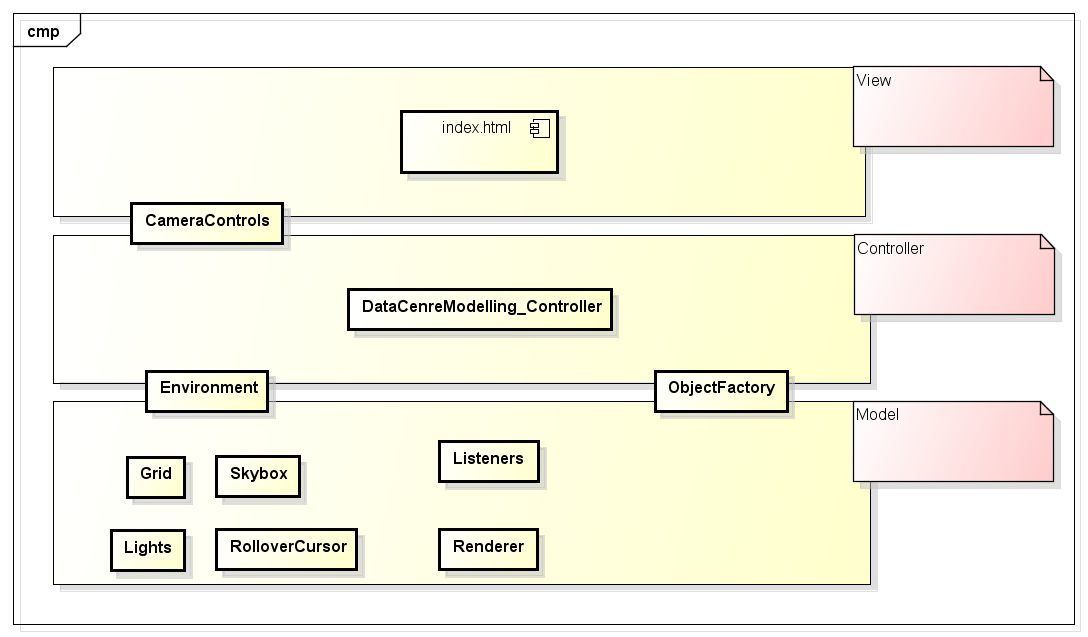
\includegraphics[width=5in]{Resources//Design_Diagrams//Component_JavaScript 3D model.png}
\caption{MVC architectural diagram of the JavaScript 3D viewer.}
\label{fig:JavaScriptArchitectureDiagram}
\end{figure}

Structurally, these classes follow a facade design pattern, with the controller class, DataCentreModelling\_Controller creating and calling the generateEnvironment method of model class Environment within it's own  method init, which is called on DataCentreModelling\_Controller's construction. 

Each one of these classes is contained within a single JavaScript file, in order to make them more intelligible to human readers, and more familiar to object-oriented programmers.

The classes Environment, Environment's subordinate classes, and ObjectFactory all contain constructors and encapsulated methods, functioning in much the same way as classes of any object oriented language, where as DataCentreModelling\_Controller behaves more like a static class; all of it's attributes are static, and many of them are accessed by other classes as static variables. This is nessecary to allow for certain things to occur by default, such as DataCentreModelling\_Controller's method init. This also allows for certain variables not to need to be re-assigned within subordinate classes, as attempts to treat them in that manner had failed.

\textcolor{red}{HERE}

\begin{figure}[H]
\centering
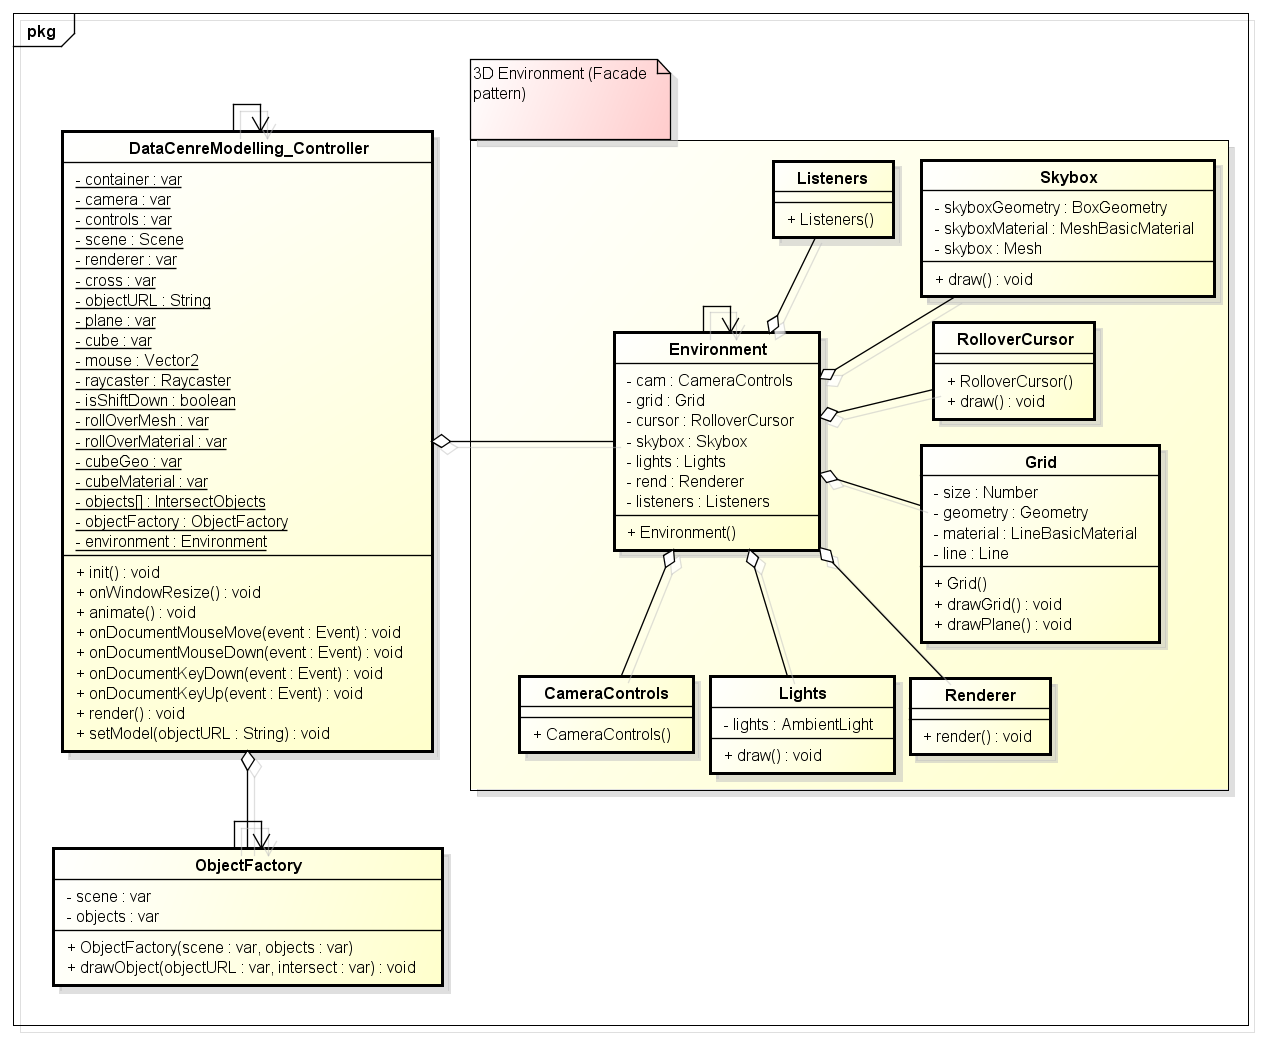
\includegraphics[width=5in]{Resources//Design_Diagrams//Class_ JavaScript Front-end.png}
\caption{UML Class diagram of the JavaScript 3D viewer. Note that due to JavaScriptbeing a weakly typed language, some attributes are labeled 'var', denoting that they are weakly typed variables. However, where a variable would have a strongly-typed analogue, such as String or into, it is labeled as such to clarify it's role. Furthermore, Where a variable is assigned as an object, even if it is not assigned that variable upon construction, is labeled as being an object of that class in order to distinguish it.}
\label{fig:ClassDiagram_JavaScriptFrontEnd}
\end{figure}

\textcolor{red}{Environment's generateEnvironment method creates objects of other classes required to generate the 3D environment, such as the grid plane, and the lights. In this role, class DataCentreModelling\_Controller constructs an object of class Environment, who's constructor constructs objects of classes required to render the 3D environment. These include those required to render certain 3D objects, such as the Grid-plane and the object placement cursor, as well as others such as the Camera-view controller object (CameraController) and listeners. As Environment does this within it's constructor, it can be thought of as a singleton class, as only a single instance of it is ever constructed, that one instance is all that is needed to render the environment, and any changes to that environment are made to the objects which were constructed by that Environment object. \textcolor{blue}{All classes called by Environment which represent 3D objects include draw methods, which are called within Environment's method init, allowing them to be constructed but not drawn if required, however, other classes required for the functionality of the environment, such as CameraControls and Listeners are fully initialised and added to the Environment object by their constructors. This can be seen in the sequence diagram of the 3D environment creation shown in figure \ref{fig:Sequence_JavaScript_create_environment}.}}

\textcolor{red}{Furthermore, the process by which the loading of the HTML page calls DataCentreModelling\_Controller, which leads to the construction of an Environment object, leading to the construction of all other objects required to render the 3D environment means that the this can be seen as a facade pattern due to a single action triggering the rendering of the whole environment. This can be seen in the JavaScript front-end class diagram in figure \ref{fig:ClassDiagram_JavaScriptFrontEnd}. \textcolor{green}{[YOU GOT THIS FAR!!!]}}

\begin{figure}[H]
\centering
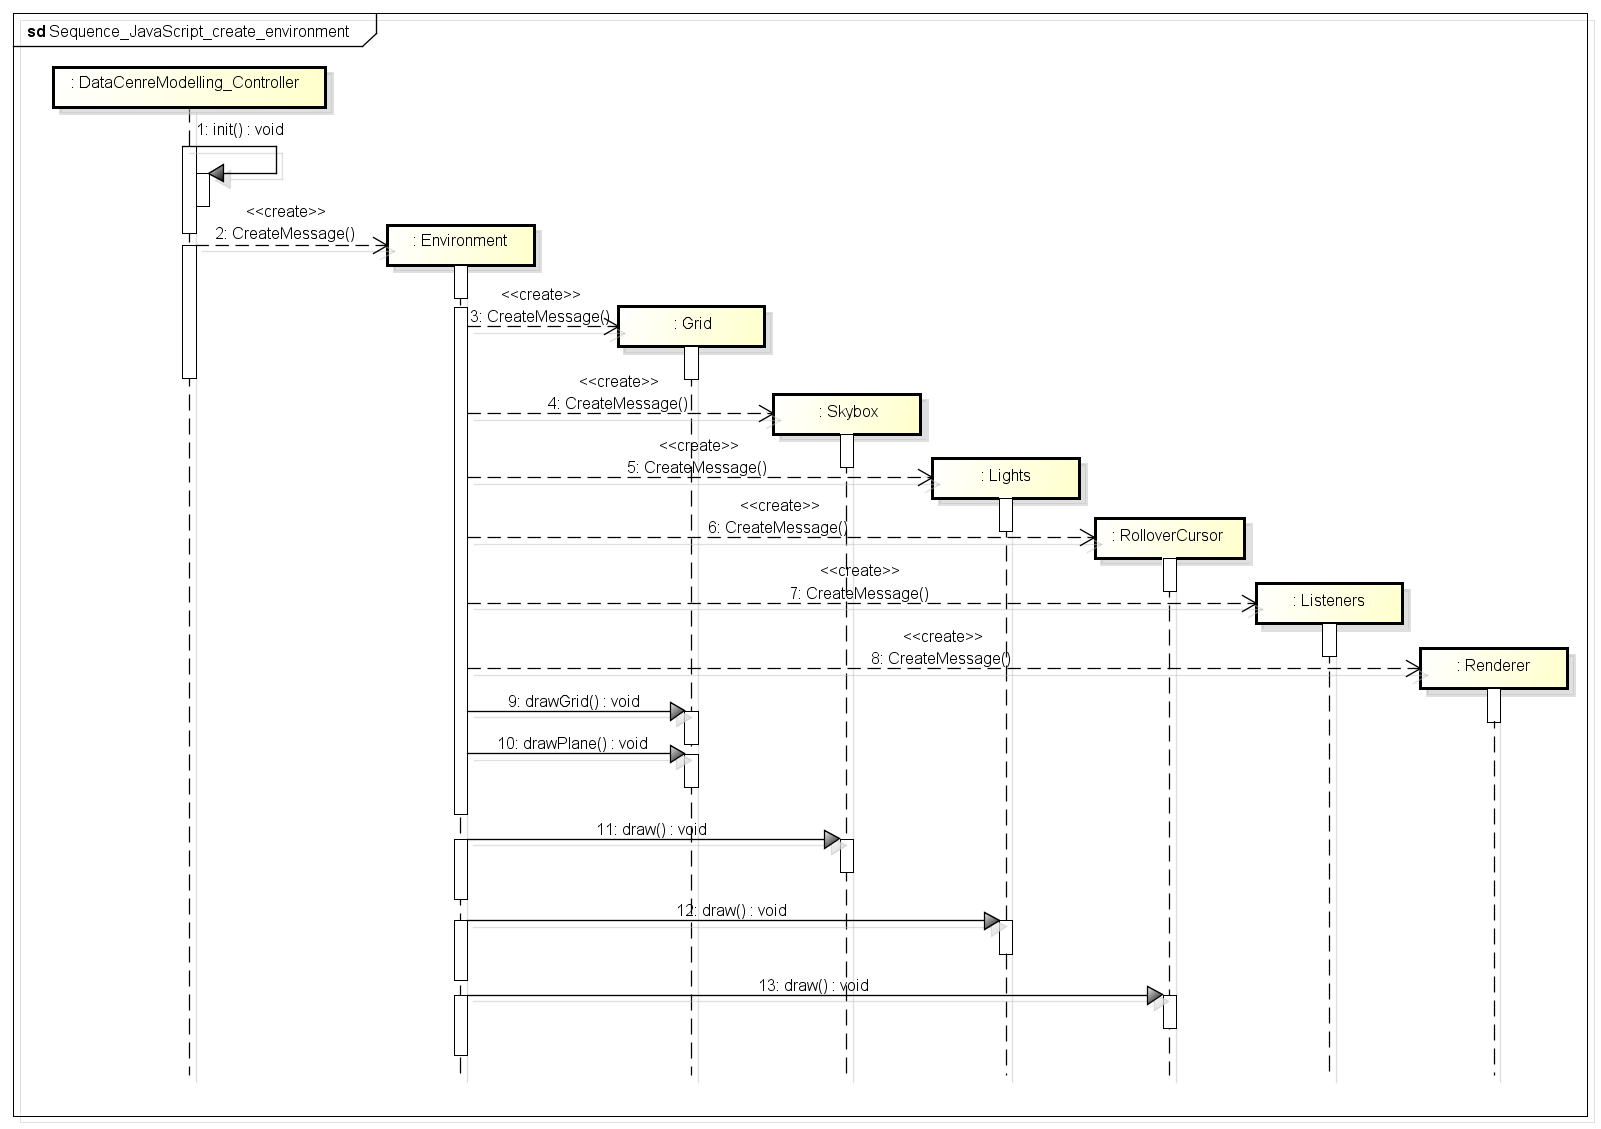
\includegraphics[width=5in]{Resources//Design_Diagrams//Sequence_JavaScript_create_environment.png}
\caption{UML Sequence diagram of the process of rendering the 3D visual environment on page load, showing interactions between JavaScript classes.}
\label{fig:Sequence_JavaScript_create_environment}
\end{figure}

\begin{figure}[H]
\centering
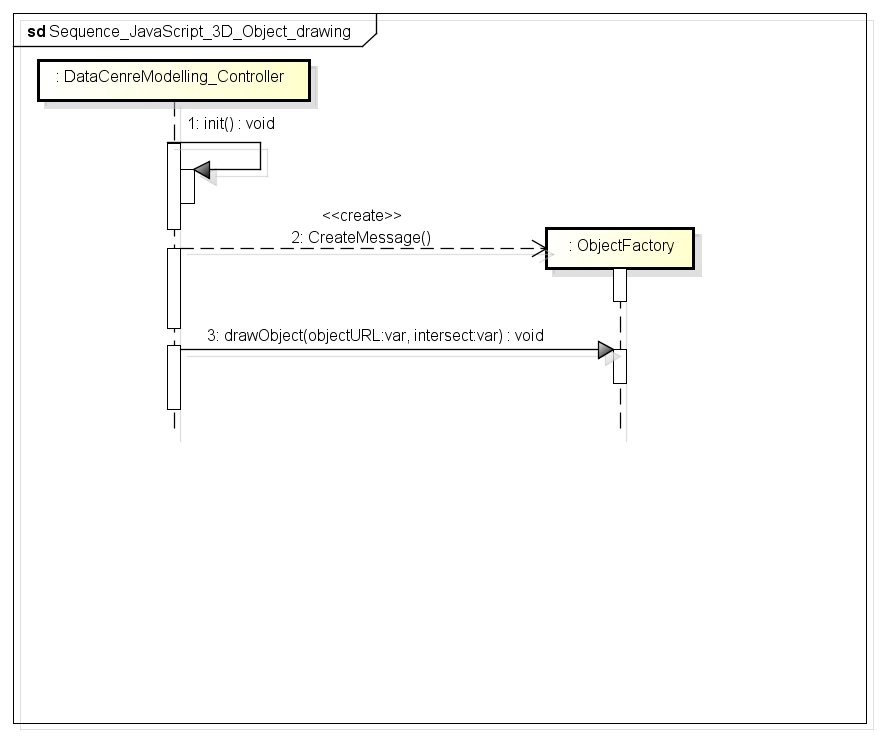
\includegraphics[width=5in]{Resources//Design_Diagrams//Sequence_JavaScript_3D_Object_drawing.png}
\caption{UML Sequence diagram of the process by which a 3D object is drawn by user interaction with the HTML view, concerning the involved JavaScript classes.}
\label{}
\end{figure}

\subsection{Back-end}

\begin{figure}[H]
\centering
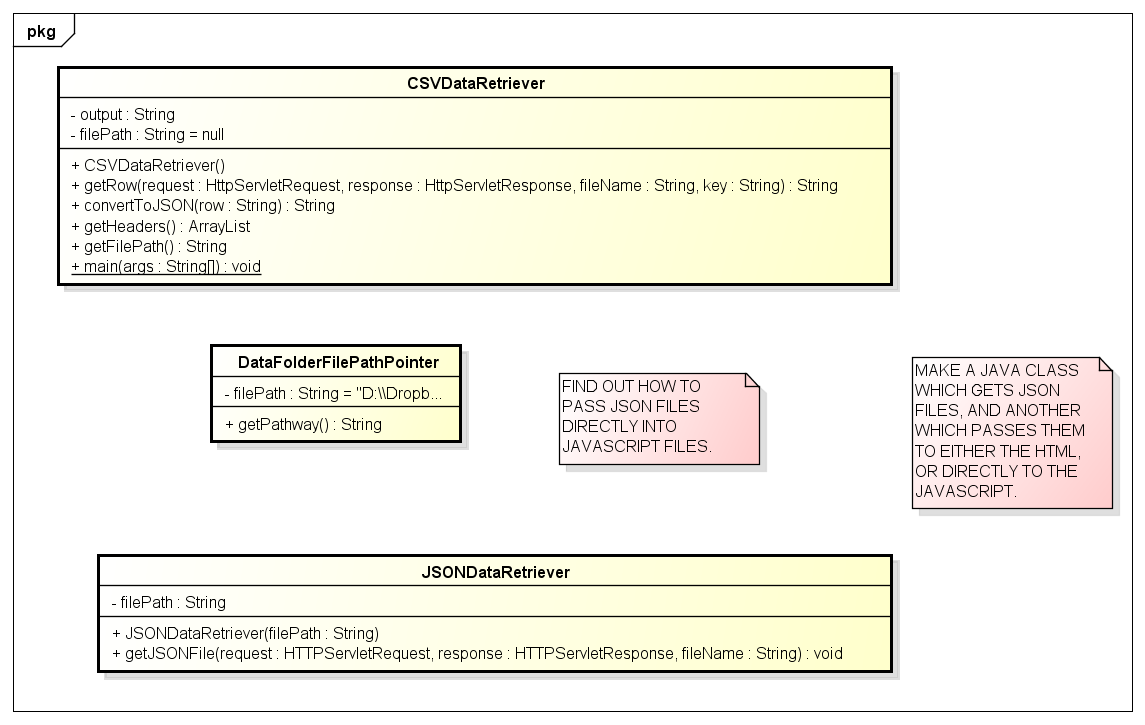
\includegraphics[width=5in]{Resources//Design_Diagrams//Class_Java Back-end.png}
\caption{}
\label{}
\end{figure}

\subsection{Support site}

\begin{figure}[H]
\centering
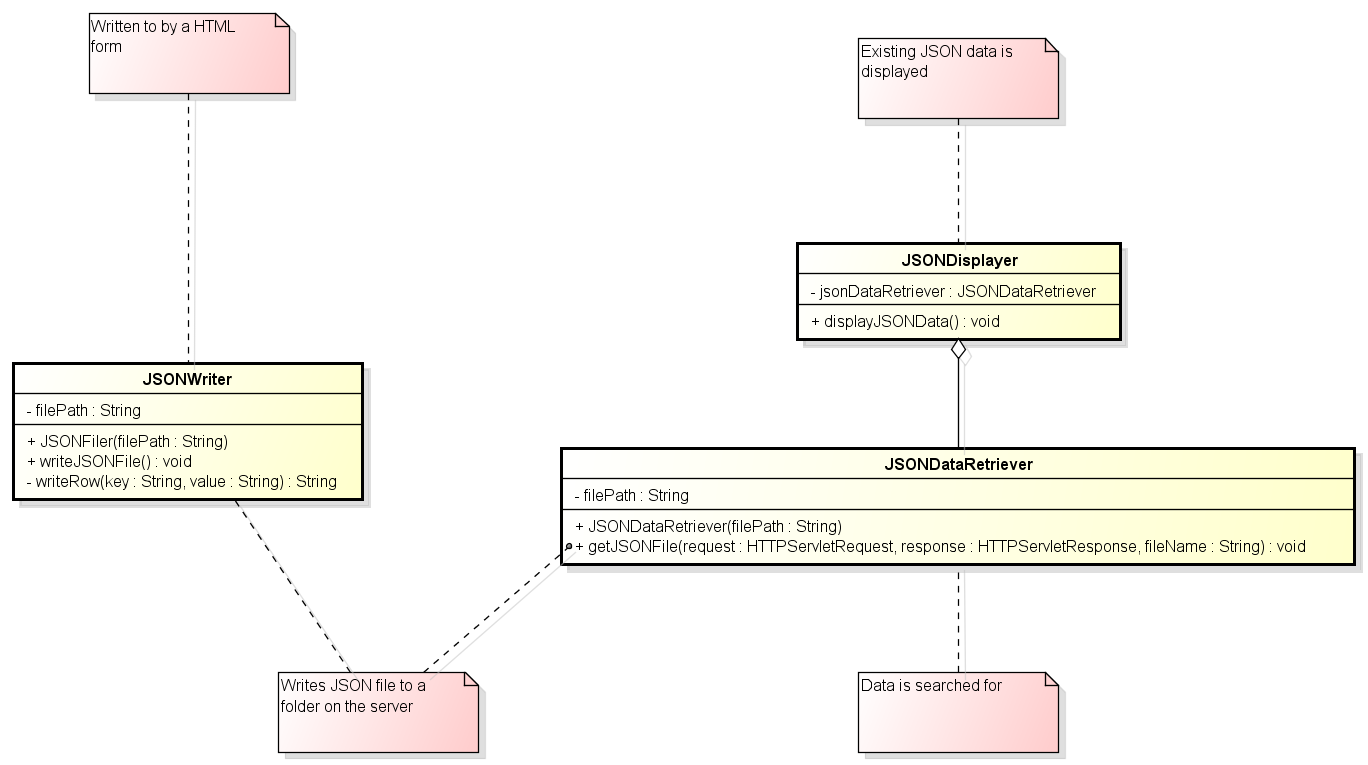
\includegraphics[width=5in]{Resources//Design_Diagrams//Class_Backend site java controller.png}
\caption{}
\label{}
\end{figure}

































%Everything else is depreciated
\iffalse

\section{Development of the Component-Database and the Logic-Engine Application Components}
\label{sec:DevelopmentOfTheComponentDatabaseAndTheLogicEngineApplicationComponents}


\subsection{Simplified Overview\textcolor{red}{[FROM PRESENTATION]}}
\label{sec:Methodology:SimplifiedOverview}
The application will be developed as a series of inter-operating sub-programs:

\begin{itemize}
\item The game interface.
    This consists of two components:
\begin{enumerate}
\item The programming interface: Ties all of the other sub-programs in the application together.

\item The Graphical User Interface, giving the user an intuitive, game like control and experience of the game
\end{enumerate}
\item The component database: containing information on anything the player can select and add to their data centre. 

\item The logic engine: A set of rules about the data centre, providing bonuses and penalties to the player based on their choices from the component database.
\end{itemize}

\begin{figure}[H]
\centering
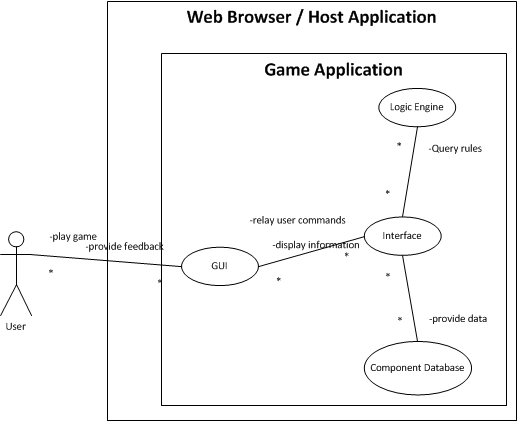
\includegraphics[width=5in]{Resources//Use Case Diagram.png}
\caption{A use-case diagram of the interactions between the sub programs.}
\label{fig:UseCaseDiagram}
\end{figure}

\subsection{Technical Overview\textcolor{red}{[FROM PRESENTATION]}}
\label{sec:Methodology:TechnicalOverview}
\subsubsection{The Component Database\textcolor{red}[FROM PRESENTATION]}
\label{sec:Methodology:TechnicalOverview:TheComponentDatabase}
This is a repository of all elements that can feasibly have an affect 
on the operation of the data centre. Examples include:

\begin{itemize}
\item Cooling systems
\item CPUs
\item Data traffic management algorithms
\item Operating times
\item Average ambient temperatures
\end{itemize}

For each of these, attributes are included, such as power
Consumption (which would be added to the overall power
consumption for the whole data-centre), purchasing cost, ideal operating 
temperature etc.

The Component Database is intended to be extensible, so that 
new technologies can be added As they become available.

Initially, an object oriented approach to the development of the database was taken
The justification of this approch is as follows:

\begin{itemize}

\item Generic classes can be used, which can be defined as being specific variations
 dependant on input parameters An example of this could be the considered to be the various
types of air conditioning system defined in section \ref{sec:ACriticalReviewOfReleventScientificAndEngineeringLiturature:StudiesIntoTheEnvironmentalEffectsAndEnergyEffiencyOfDataCenters:TheDifferentTypesOfAirConditioningEquipmentForITEnvironments}
\cite{TonyEvansTheDifferentTypesOfAirConditioningEquipmentForITEnvironmentsWhitePaper};

\item A switch-case construct could be used to define parameters supplied to an ``air conditioning system"
object at its construction, such as the devices spacial footprint, location within the room and a number 
used to define whether it is an air cooled system, a glycol cooled system, or another.

\end{itemize}

\subsubsection{Isolated testing of the Component Database}

\subsubsection{The Logic Engine\textcolor{red}{[FROM PRESENTATION]}}
\label{sec:Methodology:TechnicalOverview:TheLogicEngine}
It Will be written as a knowledge base, prototyped in a logical programming language such as Prolog or Simulink, before being written in a way that it can be used by the program interface.

Queries will consist of an entity in the Component Database being checked against the list of predicates in the Logic Engine's knowledge base. 

For example, if the user chooses a component, $A$, that has a maximum operating temperature, $T_{max}$, and then the user tries to add another component, $B$ which will raise the ambient temperature, $T_{amb}$ of the data centre above $T{max}$ , then the logic engine will prevent the Program Interface from allowing the user to add $B$.

%\begin{equation}
%\begin{split}
%&P_1 \models A \Rightarrow T_{max} \\
%&P_2 \models B \Rightarrow T_{amb} > T_{max} \\
%&C \models A \and \neg B \Rightarrow T_{amb} < %T_{max} \\
%\end{split}
%\end{equation}

\begin{equation}
\begin{split}
&P_1 \equiv A \Rightarrow T_{max} \\
&P_2 \equiv B \Rightarrow T_{amb} > T_{max} \\
&C \equiv A \land \neg B \Rightarrow T_{amb} < T_{max}
\end{split}
\end{equation}


The testing phase of this element will consist of querying a series of predicates in the knowledge base against dummy data. Once the Logic Engine works to a satisfactory extent, it will be integrated into the Testing Interface and tested against data in the Component Database.

The Logic Engine is intended to be extensible, so that if new principles are discovered that apply, they can be included.

\subsubsection{Isolated testing of the Logic Engine}

\subsubsection{The Program Interface\textcolor{red}{[FROM PRESENTATION]}}
\label{sec:Methodology:TechnicalOverview:TheProgramInterface}
This serves as the interface allowing the user to communicate with 
the program via the GUI, and for the program to query information on 
user selected components
against the logic engine.

It's development life-cycle will be in two stages:

\begin{enumerate}

\item The aforementioned “Testing Interface” will be developed in order to test the compatibility 
of the Component Database and the Logic Engine. As a test program, its input and output 
will primarily be through the command line.

\item The Testing interface will be further developed into the Program Interface by adding the
capacity for it to relay information between the other sub programs and the GUI.

\end{enumerate} 

The Program Interface will be written in JavaScript, allowing integration into a web page coded in HTML5 and CSS.

\subsubsection{Isolated testing of the Program Interface}

\subsubsection{The GUI\textcolor{red}{[FROM PRESENTATION]}}
\label{sec:Methodology:TechnicalOverview:TheGUI}
The GUI will be programmed to communicate with the program interface on the programming interface's terms. This allows multiple developments of the GUI, testing whether 2D or 3D GUIs work best with the game.

\begin{figure}[H]
\centering
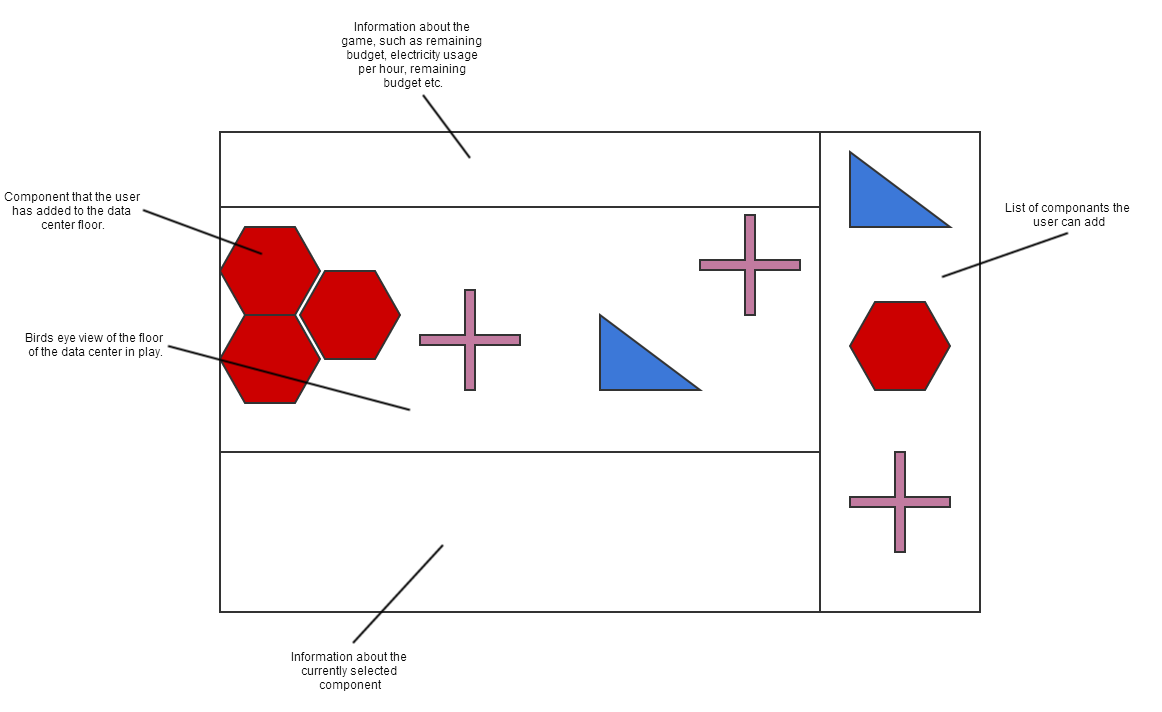
\includegraphics[width=7.25in]{Resources//GUI Mock up.png}
\caption{A mock up example of a potential GUI design, showing a top-down view of the \gls{data centre} floor, allowing users to place components from a list on the right hand side of the screen, with information about the component in the bottom pane, and general game information in the top pane.}
\label{fig:GUIMockUp}
\end{figure}

\subsubsection{Test Cycle One}
\label{sec:DevelopmentOfTheComponentDatabaseAndTheLogicEngineApplicationComponents:TestingOfTheComponentDatabaseAndTheLogicEngineViaTheTestInterface:TestCycleOne}

The first issue found was that...

This was corrected by performing the following actions:
\begin{itemize}
\item
\item
\item
\end{itemize}

The second issue found was that...

This was corrected by performing the following actions:
\begin{itemize}
\item
\item
\item
\end{itemize}

\section{Development of an Interface between the Component-Database and the Logic-Engine, and Development of a GUI}
\label{sec:DevelopmentOfAnInterfaceBetweenTheComponentDatabaseAndTheLogicEngineAndDevelopmentOfAGUI}

\subsection{Interface Development}
\label{sec:DevelopmentOfAnInterfaceBetweenTheComponentDatabaseAndTheLogicEngineAndDevelopmentOfAGUI:InterfaceDevelopment}
\textcolor{red}{The interface will be developed from the Test-Interface (section \ref{sec:DevelopmentOfTheComponentDatabaseAndTheLogicEngineApplicationComponents:TheTestInterface}). As such, this section may become obsolete and be removed.}

\subsection{The GUI}
\label{sec:DevelopmentOfAnInterfaceBetweenTheComponentDatabaseAndTheLogicEngineAndDevelopmentOfAGUI:TheGUI}
\textcolor{red}{Chronicling of the development of the GUI}

\subsection{Integration}
\label{sec:DevelopmentOfAnInterfaceBetweenTheComponentDatabaseAndTheLogicEngineAndDevelopmentOfAGUI:Integration}
\textcolor{red}{Integration of the all of the software components and the GUI together into a working program.}

\fi